
%
% Chapter Four


\chapter{RECONSTRUCTION OF THE SPECTRUM}

At RCNP, the raw data  obtained with Grand Raiden was analyzed with  a general purpose analyzer program, Tamii Analyzer, developed by A.Tamii ~\citep{Tamii-ana}.
To extract  clean and optimized spectra with the best possible resolution, events consisting of reaction products of interests without any  unwanted particles, called background, were first selected through the GR spectrometer and were transported to the focal plane. In addition to the particle positions and angles,  data measured by the detectors in the focal plane gave the ToF and energy loss  which were used to further reduce the background.
Finally,  software corrections were applied to correct higher order aberrations to improve the resolution of the spectra. All analyzed results were  stored in the HBOOK file and were plotted using the PAW and ROOT program packages from the CERN library.

\section{Particle Identification and Background Reductions}



In the (d,p) reaction at small scattering angles, most of the particles detected in the focal plane counter were protons - the particles of interests. Any other ``contamination particles'' such as unreacted deuterons and other reaction products had to be prevented from  reaching the focal plane. Neutral particles such as neutrons and $\gamma$-rays produced at the target did not make it to the focal plane through the spectrometer and were not measured by the MWDCs. Therefore, the dominant background particles  measured in this experiment were deuterons. By setting the rigidity acceptance of the spectrometer to the desired proton rigidity, most of the undesirable reaction products including deuterons did not reach the focal plane.
At RCNP, the particle identification for proton events was realized by using time-of-flight (ToF) information and the energy loss difference between the PS1 and PS2 of the GR spectrometer.


The ToF was measured as the time difference between the timing trigger from the plastic scintillator PS1 and the RF signal from the AVF cyclotron. In order to reject deuterons effectively, the corrected  ToF (denoted as RF signals in the analyzer) spectrum was used to be independent of $x_{fp}$ and $\theta_{fp}$, defined as
\begin{equation}
    \label{eq:RFC}
    \begin{aligned}
    RFC = RF - 0.130 \times x_{fp} + 22.0 \times \theta_{fp}
    \end{aligned}
\end{equation}
where RFC is the corrected ToF in channel number (ch), and $x_{fp}$ and $\theta_{fp}$ are the horizontal position in mm and horizontal angle in degree measured in the focal plane, respectively. The position and angle independence of the corrected time RFC is shown in Fig.\ref{fig:RFC}.
\begin{figure}[tpb]
  \begin{center}
    \centerline{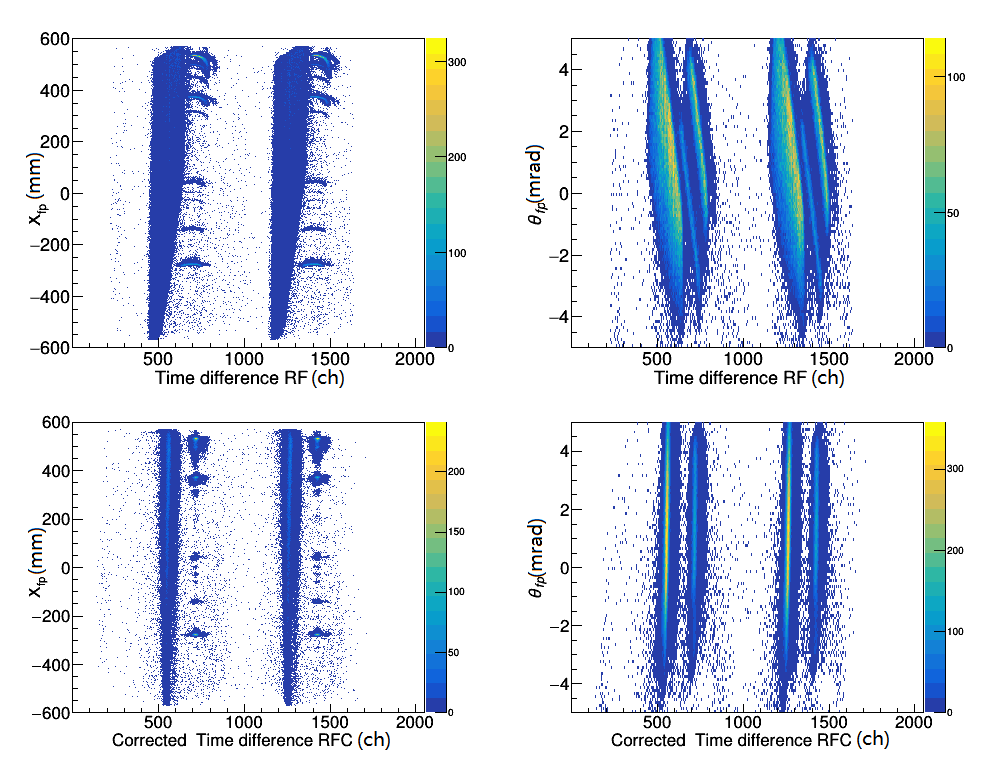
\includegraphics[scale=0.6]{graph/ch4/RFC}}
    \caption{The ToF (RF) in  the top panel and the corrected-ToF (RFC) in the bottom panel for horizontal position and horizontal angle measured at the focal plane. The corrected ToF spectra shows  the dependency on  $x_{fp}$ and $\theta_{fp}$.}
    \label{fig:RFC}
  \end{center}
\end{figure}

An independent method of particle identification is achieved by using the differences of energy losses in the two plastic scintillator detectors. When a charged particle passes through a scintillator, the energy loss depends on its charge and velocity given by the Bethe-Bloch formula:
\begin{equation}
    \label{eq:BB_formula}
    \begin{aligned}
    -\frac{dE}{dx} \propto \frac{az^2}{E}
    \end{aligned}
\end{equation}
where $z$, $a$ and $E$ refer to  the charge, mass and energy, respectively.  The energy loss of a charged particle is approximately proportional to the intensity of the light produced in the scintillator. The photons are collected by PMTs on each side of the scintillator. The number of photons arriving at each PMT depend on the position x and can be expressed in terms of the distance from the PMT $x$  as
\begin{equation}
    \label{eq:intensity}
    \begin{aligned}
    I(x) = I_0 \exp(-\frac{x}{l})
    \end{aligned}
\end{equation}
where $I_0$ is the initially produced light intensity and $l$ is the attenuation length of the scintillator. The mean intensity $I_{mean}$ measured at the left and right side of the PMTs is  expressed as
\begin{equation}
    \label{eq:intensity_mean}
    \begin{aligned}
    I_{mean} = \sqrt{I(x)I(L-x)} = I_0 \exp(-\frac{L}{2l}) \propto \Delta E
    \end{aligned}
\end{equation}
where $L$ is the length of the scintillator. As $I_{mean}$ is independent of the position of the ionization $x$, it is a useful method for particle identification. Fig. \ref{fig:PID} shows an example of particle identification using a cut in the  two-dimensional energy loss versus RFC display.


\begin{figure}[tpb]
  \begin{center}
    \centerline{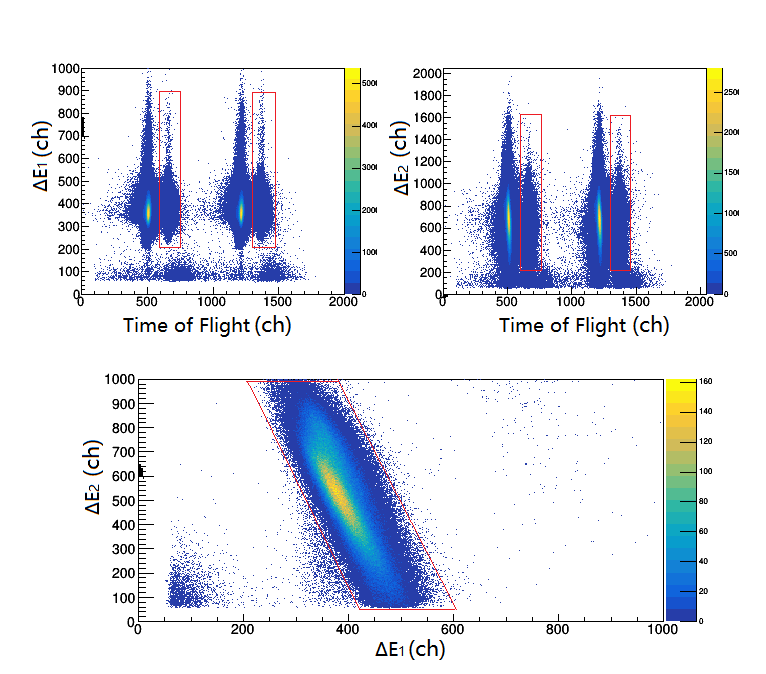
\includegraphics[scale=0.7]{graph/ch4/PID}}
    \caption{Top-left: $\Delta E_1$ vs. ToF plot. Top-right: $\Delta E_2$ vs. ToF cut. Bottom: $\Delta E_1$ v.s. $\Delta E_2$ plot. The red solid lines in these plots were event cuts  used for identifying protons and reducing background particles such as deuterons scattered off the Faraday cups inside the Dipole 1 (D1FC).}
    \label{fig:PID}
  \end{center}
\end{figure}


\section{Track Reconstruction}
As mentioned in the previous chapter, the energy of particles detected in the focal plane is determined using the kinematic equations expressed by scattering positions and angles.
The positions and angles were measured by the MWDCs in  the focal plane, which allows to reconstruct the scattering angle at the target owing to the angular dispersion matching. A voltage of -5000 V was applied to the cathode planes and -500 V to the potential wires in order to optimize the efficiency. The 6 mm spacing of the sense wires for the X-plane and 4 mm spacing for the U-plane were set at ground voltage (Fig. \ref{fig:XUplane} shows the MWDC configuration). The MWDC is designed in such a way that  the electrons, which are produced along the trajectory of a charged particle passing through, drift at a constant velocity  towards the anode under the electric field  between the cathode planes and anode wires, except for the regions nearest to the sense wire. The electrons are collected at the anode wires, generating a negative signal. Particles pass through the MWDCs at about 45$^{\circ}$ and deposit charge on 3 or 4 sense wires, called hits, as shown in Fig. ~\ref{fig:MWDCs}. In the case of a hit with three wires, the focal plane position $p$ is given by
\begin{equation}
    \label{eq:position}
    \begin{aligned}
    p=p_i+d_{sw}\frac{d_{i-1}+d_{i+1}}{d_{i-1}-d_{i+1}}
    \end{aligned}
\end{equation}
where $|d_i|$ is the minimum drift length in a cluster (adjacent to hit wires) with three wires hits, $p_i$ is the position of the $i$-th wire, $d_{i-1}$ and $d_{i+1}$ are the drift lengths to the neighboring sense wires and $d_{SW}$ is the distance between sense wires. The vertical drift lengths $d_{i-1}$, $d_{i}$, $\cdots$ were determined from the drift time recorded by the Time-to-Digital Converter (TDC) and converted to the drift lengths by drift tables. To cover all the signal wires, these drift  tables were calibrated using a spectrum in a  continuum energy region so that the drift length histogram has a flat distribution (Fig.~\ref{fig:drift_time}).


%---
%\begin{figure}[tpb]
%  \begin{center}
%    \centerline{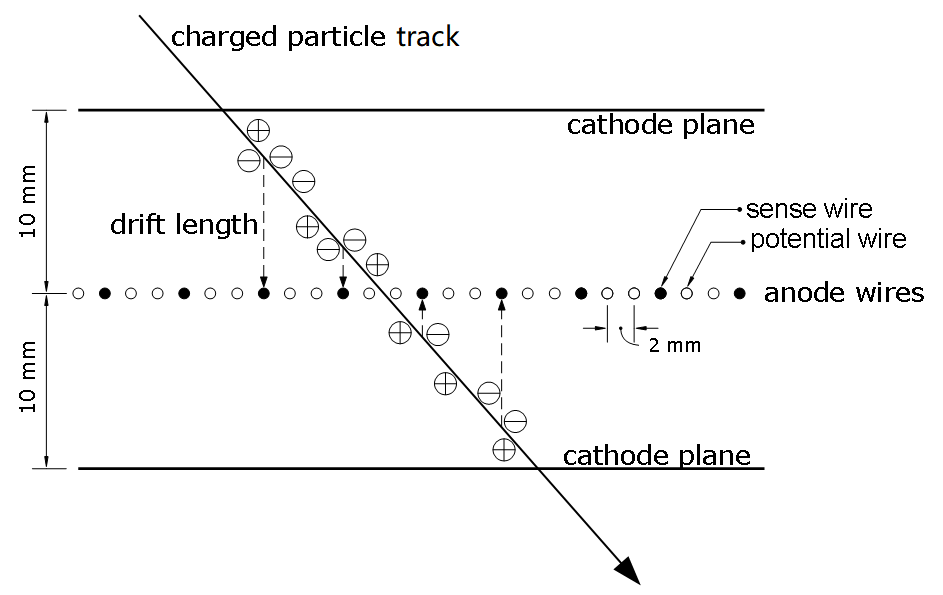
\includegraphics[scale=0.6]{graph/ch4/MWDCs_1}}
%    \caption{X-plane configuration of the MWDC. A sample of the charged particle track is shown together with the cathode planes and anode wires.}
%    \label{fig:MWDCs}
 % \end{center}
%\end{figure}
---%

\begin{figure}[tpb]
  \begin{center}
    \centerline{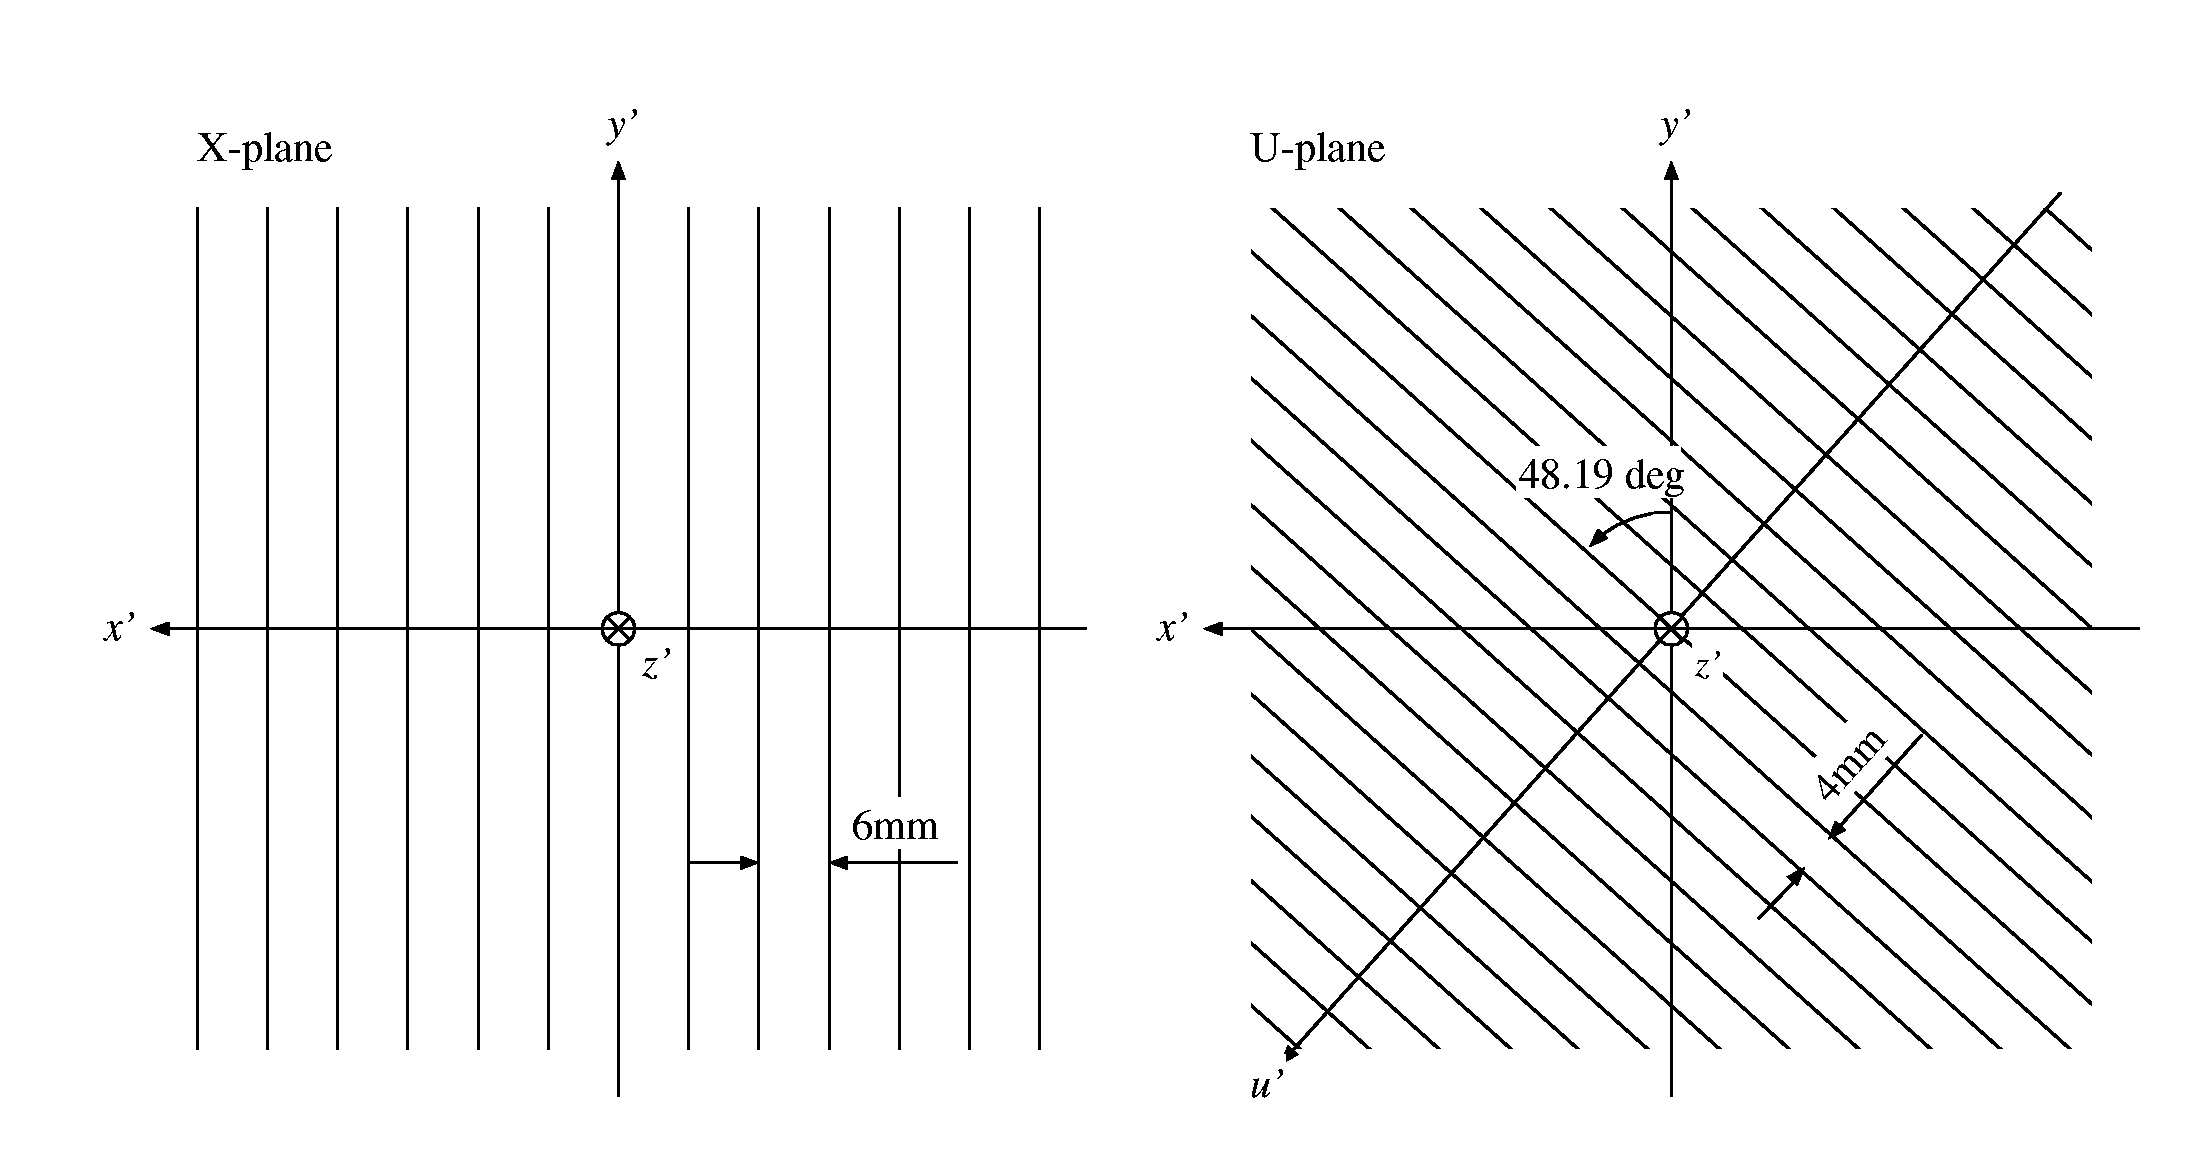
\includegraphics[scale=0.3]{graph/ch4/XUplane}}
    \caption{Wire configuration of the X-plane and U-plane of the MWDC.}
    \label{fig:XUplane}
  \end{center}
\end{figure}

\begin{figure}[tpb]
  \begin{center}
    \centerline{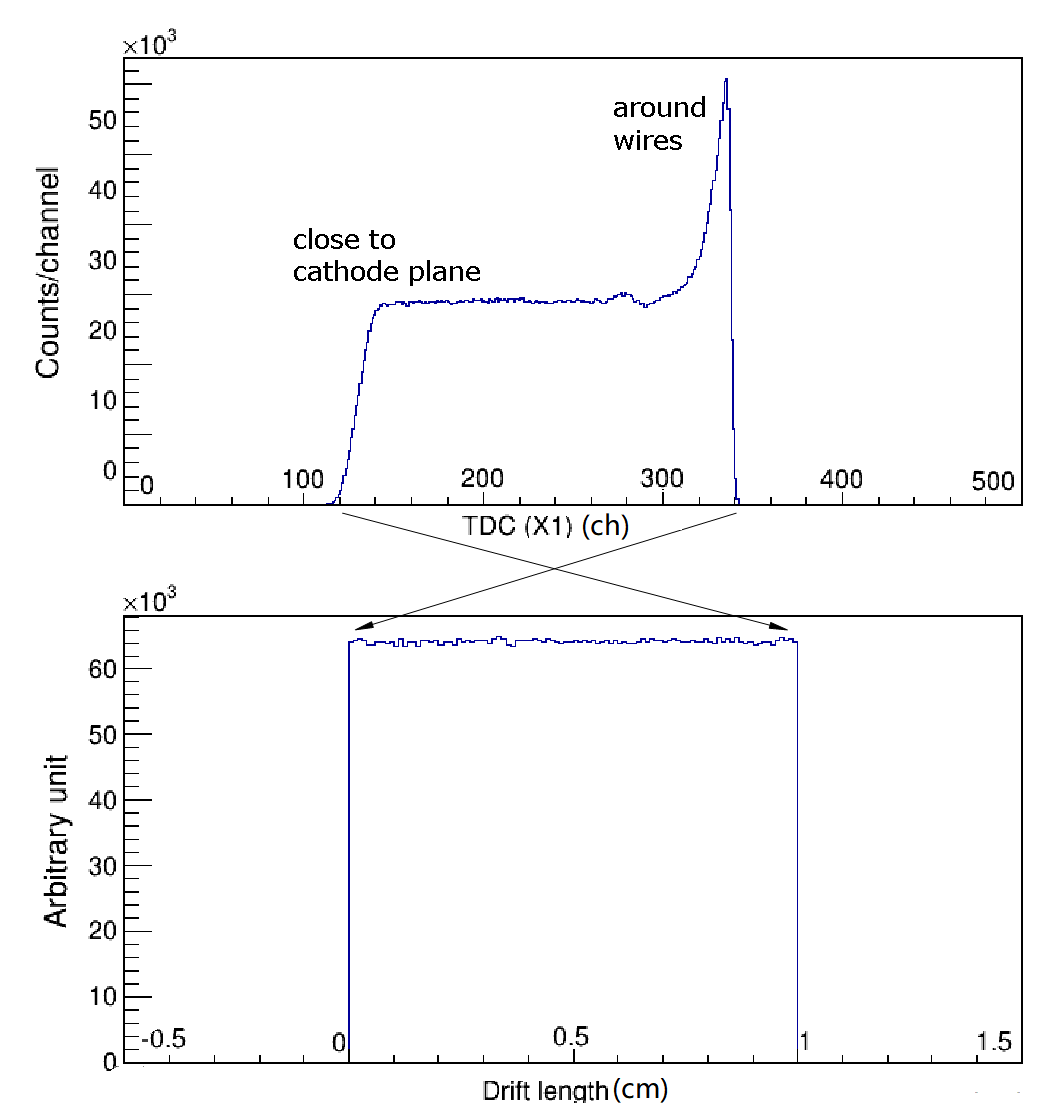
\includegraphics[scale=0.5]{graph/ch4/drift_time}}
    \caption{Conversion of the drift-time spectrum to the drift length for the position measurement with the MWDC. Example from the X-plane.}
    \label{fig:drift_time}
  \end{center}
\end{figure}

The efficiency of X1 wire plane was determined by
\begin{equation}
    \label{eq:efficiency}
    \begin{aligned}
    \eta_{X1} = \frac{N_{U1\cap X2\cap U2}}{N_{X1 \cap U1 \cap X2\cap U2}}
    \end{aligned}
\end{equation}
where $N_{X1 \cap U1 \cap X2\cap U2}$ refers to the number of events detected in all the four wire planes, and $N_{U1\cap X2\cap U2}$ is the number of events detected in the other three wire planes. The total MWDC efficiency is the product of the efficiencies of all anode wire planes:
\begin{equation}
    \label{eq:efficiency}
    \begin{aligned}
    \eta_{MWDC} = \eta_{X1} \times \eta_{X2} \times \eta_{U1} \times \eta_{U2}
    \end{aligned}
\end{equation}
In this experiment, the efficiencies for each wire plane was 96\% and the total efficiency was 85\%.



\section{Scattering Angle Reconstruction}


%%%%%%%%%%%%%
As mentioned in Section 3.3, the scattering angle of the reaction at the target $\Theta_{scatt}=\sqrt{\theta_{tgt}^2 + \phi_{tgt}^2}$ can be reconstructed from the measurement in the focal plane if the angular dispersion matching condition in horizontal direction and the off-focus mode in vertical direction  are realized, where $\theta_{tgt}$  and $\phi_{tgt}$ refer to the horizontal and vertical scattering angles, respectively. In order to calibrate the relationship between the scattering angle and the focal plane measurements, a multi-hole slit called the ``sieve-slit" (shown in Fig.\ref{fig:sieve_slits}) was placed 585 mm downstream of  the target  while the Grand Raiden spectrometer was set to 10$^{\circ}$. A gold target $^{197}Au$ with the thickness of 1.68 $mg/cm^2$ and a carbon target with a thickness of 1 $mg/cm^2$ were used in order to give spectra that cover the full range of the X-focal plane positions $x_{fp}$. The horizontal and vertical scattering angles were well defined by the geometry of the sieve-slit with respect to the target by the reactions $^{197}$Au(d,d')$^{197}$Au and $^{12}$C(d,p)$^{13}$C, respectively. As  shown in the left panel of Fig.\ref{fig:anglecalib}, the image of the sieve-slit can be seen in the focal plane by the vertical focal plane position ($y_{fp}$) versus horizontal focal plane angle ($\theta_{fp}$) for a given range of the X-focal plane position ($x_{fp}$). With the measured $x_{fp}$ and $\theta_{fp}$ from the 2-dimensional plots of images of the sieve-slit, the horizontal scattering angle $\theta_{tgt}$ was calibrated from the $x_{fp}$ and $\theta_{fp}$ dependent equation:
\begin{equation}
    \label{eq:theta_calib}
    \begin{aligned}
        \theta_{tgt} =  \sum_{i=0}^{2} \sum_{j=0}^{2}  a_{ij} \theta_{fp}^i  x_{fp}^j
    \end{aligned}
\end{equation}
The same method was used for  the vertical scattering angle $\phi_{tgt}$ calibration by the $x_{fp}$, $\theta_{fp}$ and $y_{fp}$ dependent equation:
\begin{equation}
    \label{eq:phi_calib}
    \begin{aligned}
        \phi_{tgt} = \sum_{i=0}^2 \sum_{j=0}^2 \sum_{k=0}^2 b_{ijk} \theta_{fp}^i x_{fp}^j y_{fp}^k
    \end{aligned}
\end{equation}
\begin{figure}[tpb]
  \begin{center}
    \centerline{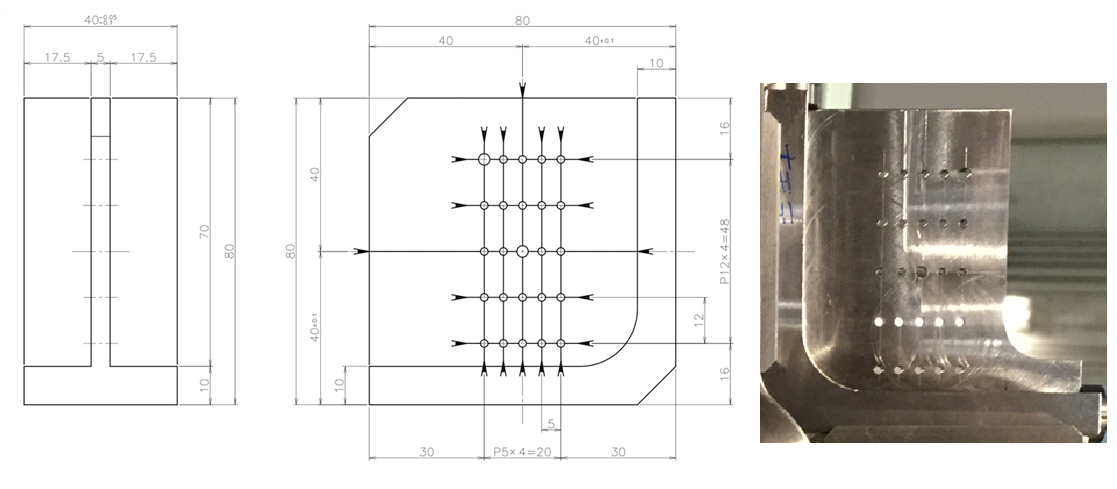
\includegraphics[scale=0.65]{graph/ch4/sieveslits_1}}
    \caption{Drawing (left side) and photograph of the sieve-slit used to calibrate the scattering angles at the target as a function of the measured focal plane angles and vertical positions.}
    \label{fig:sieve_slits}
  \end{center}
\end{figure}
where the fitting parameters $a_{i}$, $b_{i}$ , $c_{ij}$ and $d_{ij}$ were determined by a multi-dimensional non-linear least squares fit. The calibrated scattering angle from the sieve-slit pattern is shown on the right of the Fig.\ref{fig:anglecalib} as the horizontal angle versus the vertical angle. By applying the calibration equations \ref{eq:theta_calib} and \ref{eq:phi_calib} to the measurements in the focal plane ($x_{fp}$, $\theta_{fp}$ and $y_{fp}$), the horizontal and vertical components of scattering angles of the reaction products can be correlated to the target coordinates, which allows for the determination of the excitation energies populated in the recoil nucleus (parameters listed in Table.~\ref{tb:sieve-slit}).

\begin{figure}[tpb]
  \begin{center}
    \centerline{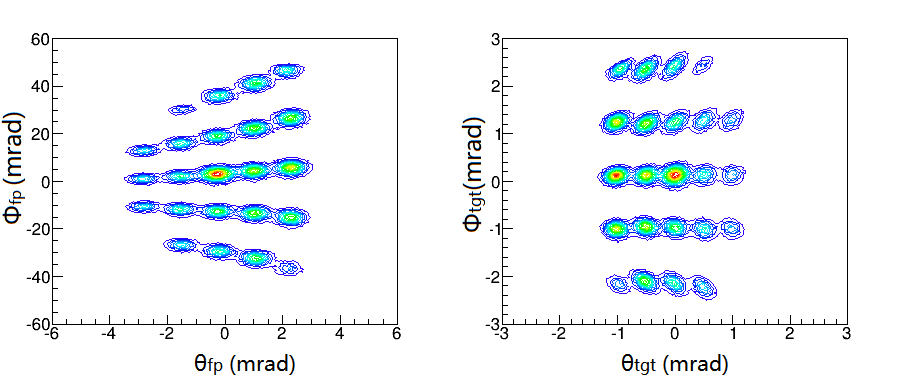
\includegraphics[scale=0.8]{graph/ch4/angle_cal}}
    \caption{2D histogram of the angular calibration run with the sieve-slit. Left panel: measurement of the vertical focal plane position ($y_{fp}$) versus horizonal angle ($\theta_{fp}$). Each blob is associated with a hole of the sieve-slit. Right Panel: reconstructed pattern at the target position after the angular calibration. Data from $^{197}$Au(d,d��)$^{197}$Au at 10$^{\circ}$.}
    \label{fig:anglecalib}
  \end{center}
\end{figure}



\begin{table}[tpb]
    \setlength{\capwidth}{0.7\textwidth}
    \begin{center}
       \caption{TABLE OF THE PARAMETERS $a_{ij}$ AND $b_{ijk}$ DETERMINED IN EQS.\ref{eq:theta_calib} AND \ref{eq:phi_calib}, RESPECTIVELY.}
       \label{tb:sieve-slit}
       \begin{tabular}{cc||cc|cc|cc}
	\hline
    \hline

    $ij$ & $a_{ij}$     & $ijk$ & $b_{ijk}$ & $ijk$ & $b_{ijk}$  & $ijk$  & $b_{ijk}$  \\
    \hline
     00  &  -2.951E+00  & 000    & -2.085E+00    &  100  &  -6.087E-01     &  200   &    2.110E-02                    \\
     01  &  6.903E+00   & 001    &  1.400E+00    &  101  &  -1.806E-01     &  201   &    1.910E-02                      \\
     02  &  4.812E-02   & 002    &  8.200E-05    &  102  &  4.091E0-05     &  202   &    1.040E-07          \\
     10  &  -2.115E-02  & 010    &  5.009E-05    &  110  &   5.000E-04     &  210   &    -3.000E-04                   \\
     11  &   2.217E-04  & 011    &  -9.012E-04   &  111  &   -3.012E-4     &  211   &    2.000E-05                   \\
     12  &   7.200E-06  & 012    &  1.031E-08    &  112  &   2.001E-07     &  212   &    2.011E-08                 \\
     20  &  -4.524E-06  & 020    &  -1.030E-06   &  120  &   8.052E-07     &  220   &    -7.000E-07                 \\
     21  &  -9.142E-08  & 021    &  3.338E-07    &  121  &   -2.019E-07    &  221   &    6.039E-08             \\
     22  &  2.694E-10   & 022    &  1.100E-09    &  122  &   7.008E-08     &  222   &    -8.000E-09                \\

       \hline
       \hline
       \end{tabular}
     \end{center}
\end{table}



\section{Software Corrections  of Higher Order Aberrations}

Besides the energy spread of the incident beam  that were corrected for the full dispersion matching conditions, there are several additional effects (higher order aberration) that need to be corrected  in order to achieve the best possible resolution.
From the reaction kinematics, it is known that particles emitted from the target at the same excitation energy of residual nucleus with different scattering angles will have different momenta $p = B\rho$ and, therefore different  magnetic rigidities $B\rho$, along with the optical aberrations,  both together hindering the spectrum resolution, especially for large angular acceptances.
These effects can be seen in the $\theta_{tgt}$ versus $x_{fp}$ plot shown on the left two panels in Fig~\ref{fig:software}. Each discrete line with curvature indicates a  state of $^{13}$C populated by the $^{12}$C(d,p)$^{13}$C reaction at 0.5$^\circ$. If projecting each curved line of events down onto the x-position, it will affect the width of the corresponding states, which is the resolution of the spectrum. Scattering particles  with larger angles are transported to the focal plane away from the scattering angle.  This creates the higher order aberrations.

The multipole magnet (MP) of Grand Raiden can be used to correct these aberration, but this  is a time consuming procedure and requires precious beam time. Therefore, to correct the kinematic effect and other higher order aberrations, software corrections were performed by straightening each discrete curved state on the 2-dimensional plots $\theta_{tgt}$ versus $x_{fp}$ and  $\phi_{tgt}$ versus $x_{fp}$ around the value of the central ray ($x_{fp}(\theta_{tgt}=0,\phi_{tgt}=0)$ in this case) using mathematical functions. The correction parameters can be determined by employing the fourth-order polynomial function:
\begin{equation}
    \label{eq:software_theta}
    \begin{aligned}
  x_{fp}'=\sum_{i=0}^2 \sum_{j=0}^4 a_{ij} x^i_{fp} \theta^j_{tgt}
    \end{aligned}
\end{equation}
and
\begin{equation}
    \label{eq:software_phi}
    \begin{aligned}
  x_{fp}''=\sum_{i=0}^2 \sum_{j=0}^4 b_{ij} x'^i_{fp} \phi^j_{tgt}
    \end{aligned}
\end{equation}
The top right plot on Fig~\ref{fig:software} shows the 2-dimensional spectrum $\theta_{tgt}$ versus $x'_{fp}$ where $x'_{fp}$ is the corrected focal plane position given by Eq~\ref{eq:software_theta}. In the analysis the horizontal component of the scattering angle was first corrected with Eq~\ref{eq:software_theta}, followed by the vertical scattering angle correction with Eq~\ref{eq:software_phi}. This procedure allowed to improve the final resolution  from 32 keV to 23 keV at 0.5$^{\circ}$ measurements.
%%%%%%%%%%%%%%%%%%%%%%%%%%%%%%%%%%%%%%%%%%%%%%%%%%%%%%%%%%%%%%%%%%%%%%%%%
\begin{figure}[tpb]
  \begin{center}
    \centerline{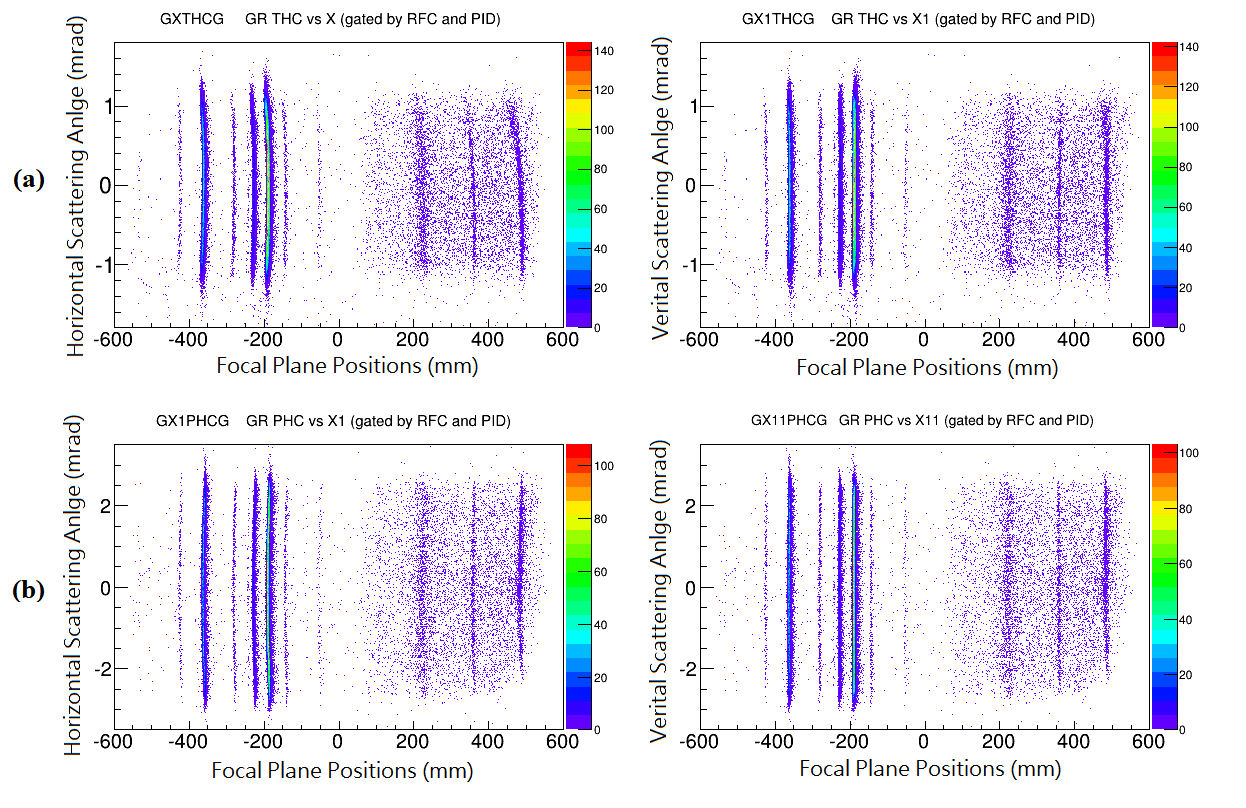
\includegraphics[scale=0.6]{graph/ch4/software}}
    \caption{Software corrections. Example of $^{12}$C(d,p)$^{13}$C at 0.5$^{\circ}$ (a) and (b): plots of the horizontal scattering angle $\theta_{scatt}$ and the vertical scattering angle $\phi_{scatt}$ versus the position in the focal plane before and after correction.}
    \label{fig:software}
  \end{center}
\end{figure}



% % uncomment the following lines,
% if using chapter-wise bibliography
%
% \bibliographystyle{ndnatbib}
% \bibliography{example}
